\let\negmedspace\undefined
\let\negthickspace\undefined
\documentclass[journal]{IEEEtran}
\usepackage[a5paper, margin=10mm, onecolumn]{geometry}
%\usepackage{lmodern} % Ensure lmodern is loaded for pdflatex
\usepackage{tfrupee} % Include tfrupee package

\setlength{\headheight}{1cm} % Set the height of the header box
\setlength{\headsep}{0mm}     % Set the distance between the header box and the top of the text

\usepackage{gvv-book}
\usepackage{gvv}
\usepackage{cite}
\usepackage{amsmath,amssymb,amsfonts,amsthm}
\usepackage{algorithmic}
\usepackage{graphicx}
\usepackage{textcomp}
\usepackage{xcolor}
\usepackage{txfonts}
\usepackage{listings}
\usepackage{enumitem}
\usepackage{mathtools}
\usepackage{gensymb}
\usepackage{comment}
\usepackage[breaklinks=true]{hyperref}
\usepackage{tkz-euclide} 
\usepackage{listings}
% \usepackage{gvv}                                        
\def\inputGnumericTable{}                                 
\usepackage[latin1]{inputenc}                                
\usepackage{color}                                            
\usepackage{array}                                            
\usepackage{longtable}                                       
\usepackage{calc}                                             
\usepackage{multirow}                                         
\usepackage{hhline}                                           
\usepackage{ifthen}                                           
\usepackage{lscape}
\begin{document}
\bibliographystyle{IEEEtran}
\title{4.2.5}
\author{EE25BTECH11002 - Achat Parth Kalpesh }
{\let\newpage\relax\maketitle}
\renewcommand{\thefigure}{\theenumi}
\renewcommand{\thetable}{\theenumi}
\setlength{\intextsep}{10pt} % Space between text and floats
\numberwithin{equation}{enumi}
\numberwithin{figure}{enumi}
\renewcommand{\thetable}{\theenumi}
\parindent 0px


\textbf{Question:}\\
Find the direction and normal vector for the line;
\begin{align}
    2x=-5y
    \label{eq:ref}
\end{align}

\textbf{Solution:}\\
Let $\vec{n}$ and $\vec{m}$ are the Normal and Direction vectors of the 
line
\begin{align}
    \vec{n_1}^\top\vec{x}=c
\end{align}
where ,
\begin{align}
    \vec{n_1} &= \myvec{2 \\ 5}\\
    c &= 0
\end{align}
The $\vec{n}$ can be represented as,
\begin{align}
    \vec{n} = \myvec{-m \\ 1}
\end{align}
Where $m$ is the slope of the line,
\begin{align}
    m &= \frac{-2}{5}\\
    \vec{n} &= \myvec{\frac{2}{5} \\ 1}
\end{align}

\eqref{eq:ref} can be represented as,
\begin{align}
    \implies \myvec{x \\ y} &= \myvec{x \\ \frac{-2}{5}x} =\myvec{0 \\ 0} + x\myvec{1 \\ \frac{-2}{5}}\\
    \implies \myvec{x \\ y} &=\myvec{0 \\ 0} + x\myvec{1 \\ \frac{-2}{5}}
\end{align}
Comparing it with ,
\begin{align}
\label{eq:geo-param}
	\vec{x} = \vec{h} + \kappa \vec{m}
\end{align}
We get,
\begin{align}
			\label{eq:line-school-dir}
\vec{m} = \myvec{1 \\ \frac{-2}{5}}
\end{align}

\begin{figure}[h]
    \centering
    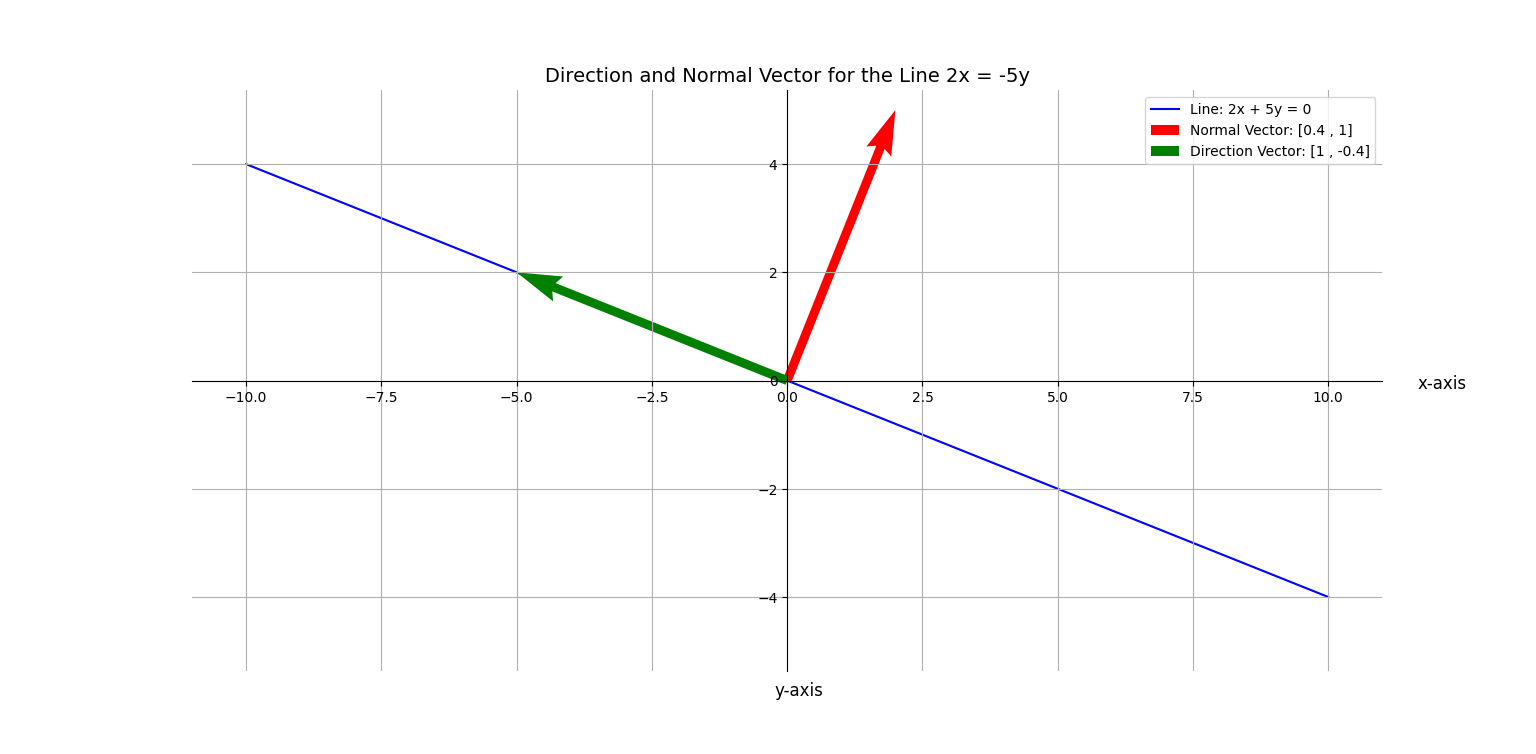
\includegraphics[width=\columnwidth]{figs/figure_py.png}
    \caption{Graph}
    \label{fig:fig}
 \end{figure}

\end{document}